\documentclass[11pt]{article}

\usepackage[margin=1in]{geometry}
\usepackage{graphicx}
\usepackage{booktabs}
\usepackage{amsmath}
\usepackage{hyperref}
\usepackage{caption}
\usepackage{float}

\title{Phase 1: Preprocessing \& Cleaning \\
\large Pan-Cancer RNA-Seq Intrinsic Dimensionality Project}
\author{}
\date{\today}

\begin{document}
\maketitle

\begin{abstract}
This report documents Phase 1 of the project ``When 20,531 Dimensions Hide a
Handful of Truths.'' It covers ingestion and integrity validation of the
TCGA Pan-Cancer RNA-Seq expression matrix ($n=801$ samples,
$d=20{,}531$ genes, 5 cancer types), the log-transform and standardization
pipeline applied prior to all downstream high-dimensional analysis, and the
variance-based feature-filtering scheme used for computationally intensive
sub-analyses in later phases. Every preprocessing decision is justified
against the statistical properties of RNA-Seq count data and the
requirements of the covariance- and distance-based methods used in
Phases 2--3.
\end{abstract}

\section{Dataset Description}

The dataset is the Gene Expression Cancer RNA-Seq collection (TCGA
Pan-Cancer Atlas, Illumina HiSeq platform), consisting of $801$ tumor
samples and $20{,}531$ gene-expression features (columns
\texttt{gene\_0}\ldots\texttt{gene\_20530}), giving an aspect ratio
$d/n \approx 25.6$. Each sample carries one of five cancer-type labels:
BRCA (breast), KIRC (kidney), LUAD (lung), PRAD (prostate), and COAD
(colon). All features are continuous, non-negative RNA-Seq expression
intensities.

\subsection{Ingestion and Validation}

The expression matrix and label vector were loaded via
\texttt{src/data\_loading.py} and validated with
\texttt{validate\_dataset()}, which asserts that the matrix shape matches
the expected $(801, 20{,}531)$, that sample identifiers in $X$ and $y$ are
aligned, and reports missing-value and zero-variance-gene counts. Table
\ref{tab:validation} summarizes the results.

\begin{table}[H]
\centering
\caption{Dataset integrity validation summary.}
\label{tab:validation}
\begin{tabular}{lr}
\toprule
Check & Result \\
\midrule
Samples ($n$) & 801 \\
Features ($d$) & 20{,}531 \\
Missing values & 0 \\
Zero-variance genes & 267 \\
\bottomrule
\end{tabular}
\end{table}

No missing values were found, consistent with the dataset documentation.
However, $267$ of the $20{,}531$ genes ($\approx 1.3\%$) have exactly zero
variance across all 801 samples --- i.e., they are recorded as a constant
expression value (in most cases zero) for every tumor sample in this
cohort. These are almost certainly genes that were not expressed, or not
reliably quantified, in any of the profiled tissue types, rather than a
data-quality artifact specific to this release.

\subsection{Class Balance}

Table \ref{tab:class-balance} and Figure \ref{fig:class-balance} report the
per-class sample counts. The dataset is moderately imbalanced: BRCA
accounts for $37.5\%$ of samples, while COAD accounts for only $9.7\%$.
This imbalance is noted here because it is a property of the raw data
(not affected by Phase 1 preprocessing), but it is directly relevant to
later phases: per-class sample counts as low as $n=78$ (COAD) constrain
the statistical power of any class-conditional geometric analysis in
Phases 2--4.

\begin{table}[H]
\centering
\caption{Class balance across the five cancer types.}
\label{tab:class-balance}
\begin{tabular}{lrr}
\toprule
Cancer type & Count & Proportion \\
\midrule
BRCA & 300 & 0.3745 \\
KIRC & 146 & 0.1823 \\
LUAD & 141 & 0.1760 \\
PRAD & 136 & 0.1698 \\
COAD & 78  & 0.0974 \\
\bottomrule
\end{tabular}
\end{table}

\begin{figure}[H]
\centering
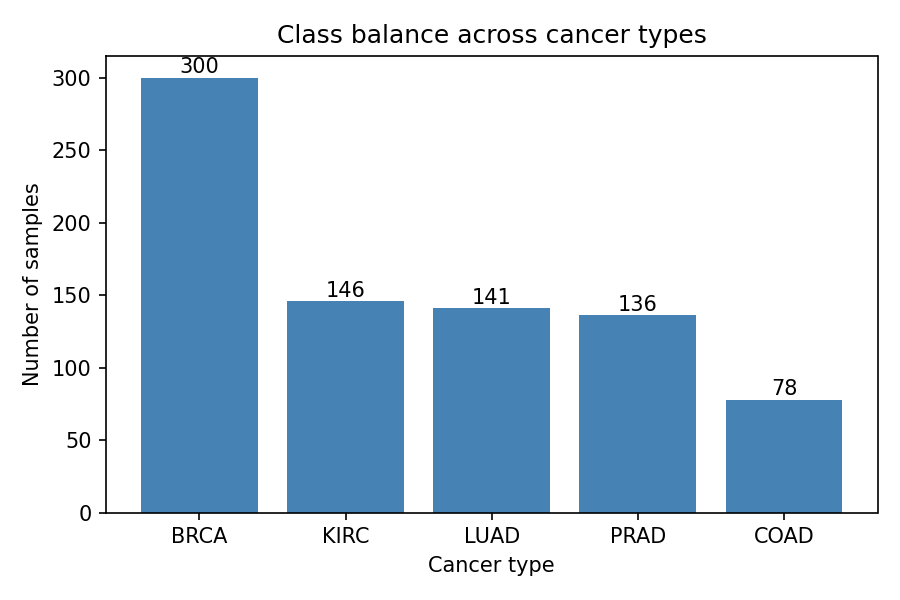
\includegraphics[width=0.7\textwidth]{../figures/class_balance.png}
\caption{Sample counts per cancer type. BRCA is the majority class
($n=300$); COAD is the minority class ($n=78$), a roughly $3.8\times$
imbalance ratio.}
\label{fig:class-balance}
\end{figure}

\section{Methodology}

Preprocessing is implemented in \texttt{src/preprocessing.py} and
orchestrated by \texttt{run\_pipeline.py} in the following fixed order:
(1) $\log_2(1+x)$-style transform, (2) removal of zero-variance genes,
(3) standardization (zero mean, unit variance), and (4) optional
variance-based filtering to the top-$k$ most variable genes for
computationally intensive sub-analyses. Steps (1)--(3) are applied to the
full retained feature set; step (4) produces a second, reduced-dimension
artifact used only where the full $20{,}531$-feature computation is
intractable (e.g., dense covariance-spectrum analysis in Phase 3).

\subsection{Log Transformation}
\label{sec:log-transform}

RNA-Seq expression counts are right-skewed: a small number of highly
expressed genes span a much larger numeric range than the bulk of
moderately or lowly expressed genes, and the raw count distribution is
approximately log-normal rather than Gaussian. This is visible in the raw
data itself and is a well-established property of sequencing count data,
arising because gene expression is fundamentally a multiplicative
(regulatory-cascade) process rather than an additive one.

Working with raw counts would violate the implicit assumptions of nearly
every downstream method used in this project: PCA and covariance-based
estimators assume features whose variance is not dominated by a handful
of extreme-magnitude outliers; Euclidean-distance-based methods (t-SNE,
UMAP, $k$-NN intrinsic-dimension estimators) would have their distance
metric overwhelmingly determined by the highest-count genes, effectively
discarding the discriminative information carried by lower-magnitude
genes. We therefore apply
\[
  X_{\log} = \log(1 + X_{\text{raw}})
\]
(the \texttt{log1p} transform, function \texttt{log\_transform()}) prior
to any other processing. Adding $1$ before taking the logarithm avoids
$\log(0) = -\infty$ for the many genes with zero expression in a given
sample, while leaving the relative ordering and approximate log-linear
scaling of larger counts intact. This is the standard transform used in
the RNA-Seq analysis literature for exactly this purpose, and it directly
addresses the skewness problem: the histograms in Figure
\ref{fig:mean-var-full} show a distribution of per-gene means with a
long-tailed but no longer extreme-outlier-dominated shape after this
transform.

\subsection{Zero-Variance Genes}
\label{sec:zero-var}

After the log transform, $267$ genes remain exactly constant across all
801 samples (Table \ref{tab:validation}). These genes carry no
discriminative information whatsoever with respect to any of the
downstream analyses in this project: they contribute a zero row/column to
every covariance or correlation matrix, cannot support any
distance-preservation argument (their coordinate never differs between
any two samples), and --- critically for the next preprocessing step ---
have zero variance, undefined under $z$-scoring (division by zero).

\textbf{Decision:} we drop all $267$ zero-variance genes
(\texttt{drop\_zero\_variance\_genes()}) prior to standardization, rather
than imputing an artificial variance or treating them as missing. This is
the only defensible choice: retaining them would either crash the
standardization step or require an arbitrary variance floor, and no
information is lost since these genes are constant by definition. The
retained feature set after this step has $20{,}531 - 267 = 20{,}264$
genes, which is used as the ``full'' feature set for all subsequent
full-dimensional Phase 1 statistics.

\subsection{Standardization}
\label{sec:standardization}

Standardization (\texttt{standardize()}) rescales every retained gene to
zero mean and unit variance,
\[
  X_{\text{scaled}, ij} = \frac{X_{\log, ij} - \mu_j}{\sigma_j},
\]
where $\mu_j$ and $\sigma_j$ are the sample mean and standard deviation
of gene $j$ computed on the log-transformed data. This step is applied
\emph{after} the log transform, not before, for two reasons. First, the
log transform is a nonlinear operation whose effect on skewness and
variance would be undone if applied to already-centered/scaled data
(log of a signed, non-count-like quantity is not meaningful for genes
whose scaled value can be negative). Second, standardization is meant to
equalize the \emph{already-approximately-log-normal} per-gene scales
produced by the log transform, not to compensate for the raw-count-scale
skewness itself --- that is the log transform's job.

Standardization is critical for two distinct classes of downstream
method used in Phases 2--3:

\begin{itemize}
  \item \textbf{Covariance-based methods} (PCA, the empirical spectral
  distribution / Marčenko--Pastur comparison in Phase 3): without
  standardization, genes with the largest raw variance would
  dominate the sample covariance matrix and its leading eigenvectors
  purely as an artifact of measurement scale, not because they carry
  more biological signal. Standardizing first ensures PCA operates on
  the correlation structure between genes rather than being driven by a
  handful of high-variance features.
  \item \textbf{Distance-based methods} (t-SNE, UMAP, $k$-NN intrinsic
  dimension estimators, the Grassberger--Procaccia correlation
  integral): Euclidean distance is scale-sensitive by construction. If
  features are left on heterogeneous scales, pairwise distances --
  and therefore every neighborhood, embedding, and correlation-dimension
  estimate computed from them -- would be dominated by whichever genes
  happen to have the largest post-log variance, regardless of their
  true contribution to the biological separation between cancer types.
\end{itemize}

Because both categories of method are used extensively in this project,
we standardize once, consistently, immediately after the log transform
and zero-variance filtering, and use the same standardized matrix as the
common input to every downstream analysis in Phases 2--3.

\subsection{Variance-Based Feature Filtering}
\label{sec:filtering}

Several Phase 3 analyses (e.g., the dense empirical covariance spectrum
used for the Marčenko--Pastur comparison) are computationally
intractable, or at least impractical for iterative exploratory work, at
the full $d = 20{,}264$ dimensionality. We therefore additionally produce
a reduced-dimension artifact by keeping only the
$k = 2{,}000$ most variable genes (\texttt{filter\_top\_variable\_genes()},
threshold set in \texttt{src/config.py} as
\texttt{N\_TOP\_VARIABLE\_GENES}), ranked by variance computed on the
log-transformed (pre-standardization) data.

Two details of this design are worth making explicit. First, variance is
ranked on the log-scale data, \emph{not} on the standardized data: after
standardization every gene has unit variance by construction, so ranking
post-standardization variance would be meaningless. Second, $k=2{,}000$ is
used only as a computational-tractability subset for specific
sub-analyses flagged in later phases; per the project specification, every
full-dimensional computation that is feasible (including all of this
phase's exploratory statistics) is reported on the complete
$20{,}264$-gene set as well, so that the reduced-feature variant is never
presented as a substitute for the full result, only as a supplement where
strictly necessary. The threshold $k=2{,}000$ was chosen as a round number
large enough to retain substantially more genes than any known pathway or
co-expression module while remaining small enough for dense $O(k^2)$
covariance computation and iterative visualization work; it is not
intended as a claim about the true intrinsic dimensionality of the data
(that claim is the subject of Phase 2).

\section{Exploratory Results}

Figure \ref{fig:mean-var-full} shows the distribution, across all
$20{,}264$ retained genes, of per-gene mean and per-gene variance on the
log-transformed (pre-standardization) scale. The mean distribution is
bimodal: a cluster of genes near zero (lowly/rarely expressed genes,
consistent with the many small but nonzero counts remaining after
dropping only the strictly-zero-variance genes) and a broad mode around
$\log(1+x) \approx 2$--$2.5$ (moderately-to-highly expressed genes). The
variance distribution is heavily right-skewed even after the log
transform: the majority of genes have small variance across samples
(similar expression level regardless of cancer type), while a
long tail of genes shows substantially higher variance --- these
high-variance genes are the candidates most likely to carry
cancer-type-discriminative signal, and are exactly the genes prioritized
by the top-$k$ filtering scheme of Section \ref{sec:filtering}.

\begin{figure}[H]
\centering
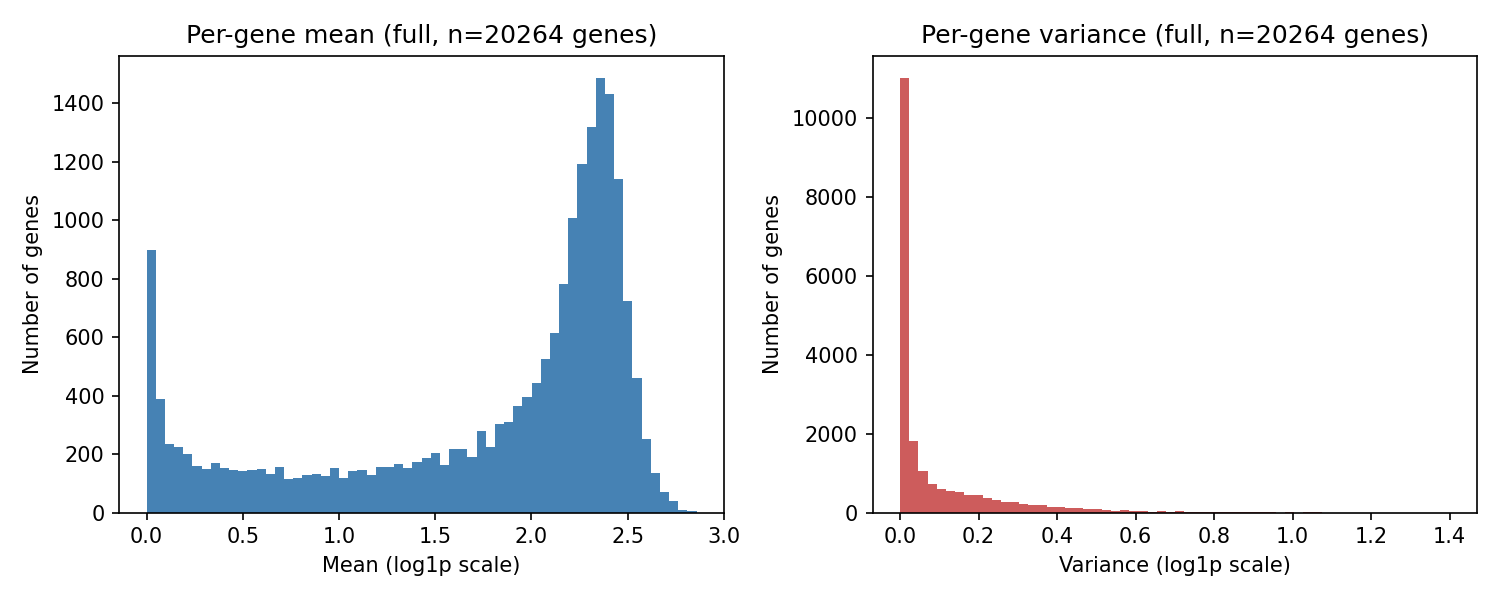
\includegraphics[width=\textwidth]{../figures/gene_mean_variance_full.png}
\caption{Per-gene mean (left) and per-gene variance (right) on the
log-transformed scale, full retained feature set ($n=20{,}264$ genes,
zero-variance genes already excluded).}
\label{fig:mean-var-full}
\end{figure}

Figure \ref{fig:mean-var-topk} shows the same statistics restricted to the
top-$2{,}000$ most variable genes selected in Section
\ref{sec:filtering}. As expected by construction, the variance
distribution is shifted substantially higher (minimum variance in this
subset is, by definition, at least the $2{,}000$th-highest variance in the
full set), while still exhibiting a right-skewed shape -- confirming that
even within the ``high-variance'' subset, variance is not uniformly
distributed, and a further, smaller core of especially high-variance
genes exists.

\begin{figure}[H]
\centering
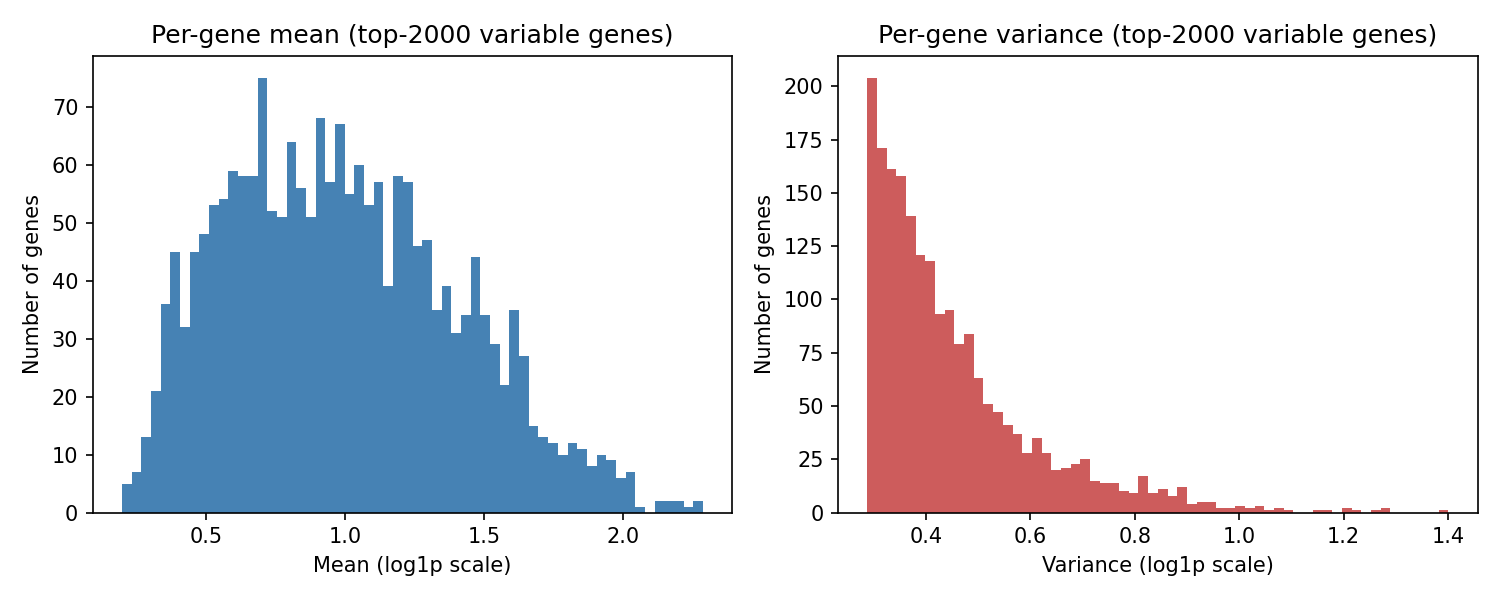
\includegraphics[width=\textwidth]{../figures/gene_mean_variance_topk.png}
\caption{Per-gene mean (left) and per-gene variance (right) on the
log-transformed scale, restricted to the top-$2{,}000$ most variable
genes.}
\label{fig:mean-var-topk}
\end{figure}

\section{Processed Artifacts}

The following intermediate artifacts are cached to \texttt{data/processed/}
by \texttt{run\_pipeline.py} for reuse by later phases, avoiding
recomputation of the (comparatively expensive) full-matrix log-transform
and standardization steps:

\begin{itemize}
  \item \texttt{phase1\_full.npz}: standardized, log-transformed,
  zero-variance-filtered expression matrix ($801 \times 20{,}264$) and the
  boolean gene-retention mask relative to the original $20{,}531$ columns.
  \item \texttt{phase1\_topk.npz}: standardized top-$2{,}000$-variable-gene
  matrix ($801 \times 2{,}000$) and the integer indices (into the
  $20{,}264$-column full matrix) of the selected genes.
  \item \texttt{labels.csv}: the aligned cancer-type label vector.
  \item \texttt{validation\_summary.json}: the full validation report
  (Table \ref{tab:validation}), including the complete list of dropped
  zero-variance gene names.
\end{itemize}

\section{Summary}

Phase 1 establishes a single, well-justified preprocessing pipeline ---
log transform, zero-variance-gene removal, standardization, and optional
variance-based filtering --- that is applied consistently ahead of every
covariance-based and distance-based method used later in the project.
The dataset has no missing values but $267$ constant genes, which are
removed rather than imputed. Standardization is applied strictly after
the log transform so that the two steps address distinct problems
(distributional skewness versus heterogeneous per-gene scale) without
interfering with each other. A top-$2{,}000$-variable-gene reduced
representation is produced solely for computational tractability in later
phases and is reported alongside, never instead of, full-dimensional
results.

\end{document}
